
\chapter{Self-attentive knowledge tracing}
	\begin{figure}[!htb]
		\centering
		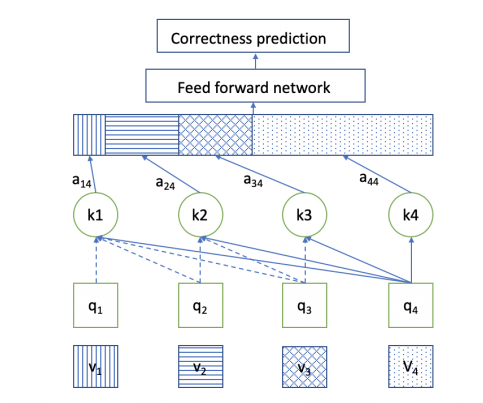
\includegraphics[scale=0.8]{sakt1.png}
		\caption{}
		\label{}
	\end{figure}
	Pronađen je rad koji istražuje novi smjer knowledge tracinga \url{https://github.com/TianHongZXY/pytorch-SAKT}. Predloženi model SAKT prvo identificira relevantne koncepte znanja iz prošlih interakcija te predviđa korisnikove performanse na tim konceptima. SAKT daje težinske vrijednosti prethodno odogovorenim pitanjima. U radu se tvrdi da je prema AUC bolji za 4.43\% od state-of-art metoda uprosječeno po svim korištenim skupovima podataka. Također, glavna komponenta (self-attention) se može paralelizirati što daje znatnu prednost po brzini naspram modela temeljenih na RNN-ovima.

		\begin{figure}[H]
		\centering
		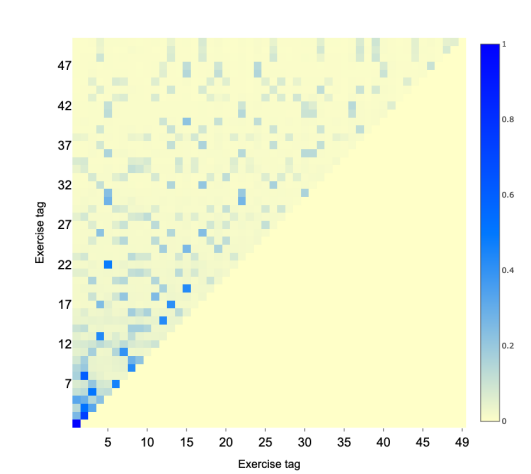
\includegraphics[scale=0.8]{sakt2.png}
		\caption{Izračunata matrica relevantnosti između zadataka}
		\label{}
	\end{figure}
	\begin{figure}[!htb]
	\centering
	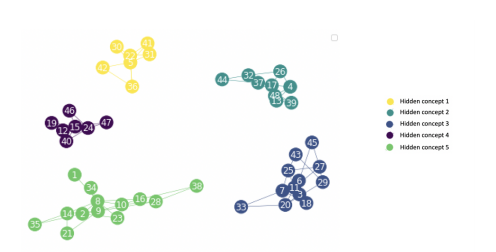
\includegraphics[scale=0.8]{sakt3.png}
	\caption{Pronađeni latentni koncepti}
	\label{}
\end{figure}

	\section{Općenito o funkcioniranju attention modela}
	Bit mehanizama pažnje (engl. \textit{attention mechanism}) je što su oni imitacija mehanizma ljudskog vida. Kad vid detektira objekt, tipično ne skenira cijelu scenu nego se fokusira na određeni dio koji odgovara osobnim potrebama promatrača. Kad osoba primijeti da se željeni objekt tipično pojavljuje u određenom dijelu scene, naučit će se u budućnosti fokusirati na takve dijelove.

	Ovakvi mehanizmi najčešće su korišteni u obradi prirodnog jezika. Izračunavanje pažnje u računalnom smislu može se opisati kao mapiranje upita (engl. {query}) i skupova parova ključ-vrijednost (engl. {key-value}) izlazu. Prvo se uzmu upit i svaki ključ te se računa sličnost među njima kako bi se dobila težina. Kao funkcija sličnosti najčešće je korišten skalarni produkt. Drugi korak je provođenje normalizacije tih težina, najčešće softmax funkcijom. Potrebno je povezati težine s odgovarajućim vrijednostima. Rezultat je konačna pažnja. 

	Modeli pažnje u potpunosti zamjenjuju RNN. Koristi se Multi-head Attention Mechanism. Postoje i slojevi s unaprijednom propagacijom te rezidualni sloj za bolju optimizaciju (koristi Add\&Norm).

	Koncept pažnje skaliranog skalarnog produkta (engl. \textit{Scaled Dot-Product Attention}) za račun sličnosti koristi skalarni produkt, kao što je spomenuto u prijašnjem tekstu. Ima dodatnu dimenziju za prilagodbu koja onemogućava da unutarnji produkt postane prevelik.

	Kod Multi-Head Attention strukture upit, ključ i vrijednost prvo prolaze linearnu transformaciju i onda u račun pažnje skaliranog skalarnog produkta. Pažnja se računa $h$ puta, otuda naziv Multi-Headed.  Svaki put kada upit, ključ i vrijednost prolaze linearnu transformaciju, mijenja se parametar W, koji predstavlja težine. Rezultait $h$ iteracija skaliranog skalarnog-produkta spajaju se na kraju.


	\section{Problemi sa SAKT-om}
	Za vrijeme pručavanja i prilagođavanja SAKT-a našim potrebama naišli smo na puno grešaka i nejasnih linija koda. Najveći problem je slaba dokumentacija koda, nedostatak originalnog dataseta te manjak iskustva sa PyTorchom.
	Na kraju smo odlučili odustati od SAKT-a zbog manjka vremena. PyTorch na različite načine izvršava operacije s CPU i CUDA tenzorima. Gradijenti treniranja na CUDI mogu se prosljeđivati slojevima samo za operacije s tenzorima, ali ne s ostalim tipovima podataka. Imali smo problem što kod zahtijeva grafičke kartice (GPU CUDA) koje naši laptopi nemaju, a debug mode ne postoji na Google Colabu. Također, dosta često Colab ne ispisuje print() funckije koje dolaze prije exceptiona tako da nismo ni na taj način mogli tražiti greške. U sljedećem potpoglavlju su nabrojane greške, neodumice i kako smo ih ispravljali ako će netko u budućnosti opet proučavati taj kod.
	\subsection{Greške i ispravci}
	
		U funkciji getitem skripte dataset.py se kod uzimanja listi nekad izbacuju prvi/ zadnji članovi ([1:],[:-1]), pošto to nema logike izmjena je takva da se uzima cijela lista ([:]). U datasetu se uzima num\_skill kao najveći index u listi zadataka te se kasnije svugdje u programu stavljalo +1, to je izmijenjeno tako da se gleda broj zadataka te je maknut +1. U dodavanju podataka u varijablu 'x' su se dodavale True /False vrijednosti što je bacalo grešku te je sada 1/0. Također nije jasno zašto se na 'x' appendaju točnosti problema onoliko puta koliko i postoji različitih zadataka. U klasi DataPrefetcher dolazilo je do greške gdje objekt lista nema metodu .to(device=self.device, non\_blocking=True). Pronađeno je da se takva metoda može pozivati nad objektom Tensor te je iskorištena metoda torch.cat().
		
		Nadalje se javlja greška u skripti run.py, funkciji run\_epoch - "can't convert cuda:0 device type tensor to numpy. Use Tensor.cpu() to copy the tensor to host memory first.". Tamo je potrebno sve varijable čije su memorijske lokacije na grafičkoj kartici zbog CUDA operacija vratiti na procesor (npr. problems.cpu()).
		
		Daljnje greške nisu mogle biti ispravljene zbog nepoznavanja što bi ti dijelovi koda trebali raditi. Primjerice u istoj metodi kod ugniježdenih petlji ima pozivanja size(1) koji je zapravo nepostojeći te se dobiva greška da se očekuje 0 ili -1, također prema izgledu petlje čini se kako bi dodavanje offseta kroz neko vrijeme dovelo do indeksa koji su veći od maksimalnog za dana polja/tensore. Kako bi se to izbjeglo, zakomentirane su originalne linije pristupanja elementima te se umjesto iteriranja po listi i dodavanja ta ista lista appenda na drugu.
		
		Sljedeća greška se događala u student\_modelu gdje se zbrajaju dva tensora različitih veličina - "output with shape [50400, 200] doesn't match the broadcast shape [1, 50400, 200]", kako bi se maknula dimenzija "1" nad tim objektom je napravljena operacije unsqueeze(0).
		
		Greška koju nismo uspijeli ispraviti je "CUDA error: CUBLAS\_STATUS\_ALLOC\_FAILED when calling `cublasCreate(handle)",te dolazi u
		retku" res = self.multi\_attn(query=self.layernorm(problems), key=x, value=x,key\_masks=None, query\_masks=None, future\_masks=None)" ono što smo uspijeli saznati je da to vrlo vjerojatno dolazi kada embedding layer dobiva krive indekse i izađe izvan intervala legalnih indeksa, odnosno, moguće je da postoji nekonzistentnost između broja oznaka i broja izlaznih jedinica sloja.
		
	\section{Sakt \#2}
		Pronađen je još jedan github repozitorij \url{https://github.com/thosgt/kt-algos} koji u sebi ima implementaciju SAKTA-a. Također uz to ima implementaciju DKT-a i još neke pomoćne skripte. SAKT dio je prilagođen da se može pokretati za assistments i biologiju na Google Colabu. Za assistments se dobivaju velike vrijednosti AUC za vrijeme treniranja što je se poklapa sa prethodnim radom. Trenutno još nije sigurno kako bi se predikcije iz SAKT-a mogle iskoristiti za preporuku sadržaja.
	
		\subsection{Generiranje candidate-exercises}
		Dio SAKT-a za vrijeme učenja razvija tako zvanu attention matricu. Ona modelu daje neku mjeru "relevantnosti" između pojedinih zadataka. Ideja je izvući tu matricu iz modela i iskoristiti njene vrijednosti za uzimanje dijela zadatka kao potencijalnu preporuku u ExRec-u. Napravljena je klasa koja prima attention matricu, funkciju normalizacije, funkciju praga te vrijednost praga. Funkcija normalizacije služi kako bi se svaki redak matrice normalizirao po nekom pravilu i onda kasnije uz pomoć funkcije praga odredili zadaci za preporuku. Klasa je napravljena tako da neće preporučiti zadatke koji su već bili. 

		Eksperimentirano je s vremenom uzimanja vrijednosti attention matrice. Uzimanje je postavljeno nakon svakog \textit{train\_batcha} i na kraju faze treniranja. Problem je što bi se, zbog korištenja softmax normalizacije pri preporučivanju, vrijednosti u pojedinim retcima trebale postaviti unutar intervala [0, 1], no to nije slučaj. Trenutno razmišljanje je da je to zbog izbacivanja nepotrebnih dimenzija tenzora. Zbog manjeg poznavanja PyTorch funkcionalnosti i načina ophođenja s visokodimenzionalnim tenzorima, moguće je da dimenzije okarakterizirane kao nepotrebne zapravo to nisu.

		Softmax je inače preporučen kao funkcija koja se koristi pri problemima multinomijalne klasifikacije (u više od dvaju klasa), a kod binarne klasifikacije češće je korištena sigmoida. Potrebno je još ispitivanja i isprobavanja raznih kombinacija funkcija i pragova.
		
	\section{Poveznice}
\url{https://medium.com/@Alibaba_Cloud/self-attention-mechanisms-in-natural-language-processing-9f28315ff905}
\url{https://towardsdatascience.com/illustrated-self-attention-2d627e33b20a}
\url{https://www.geeksforgeeks.org/activation-functions-neural-networks/}
